\chapter{作成したプロンプト}\label{cha:Proposal}

本章では、第1章で述べた課題を解決するために本研究で作成した、システム仕様書章立て生成プロンプトについて述べる。

\section{プロンプトの構成}

\begin{figure}[H]
  \centering
  \includegraphics[width=0.9\linewidth]{images/prompt_figure.pdf}
  \caption{プロンプト作成の全体像と構成要素}
  \label{fig:prompt_structure}
\end{figure}


本プロンプトの作成には、Jules Whiteらによるプロンプトパターンカタログ\cite{prompt-engineering}を参考にした。
本プロンプトは、図\ref{fig:prompt_structure}のように、役割付与、ベース章立て、システム情報、システム仕様書の定義、出力指示の５つの要素から構成されている。

プロンプトの全文を図\ref{fig:prompt_full_text}に示す。

\begin{tcolorbox}[
  colback=white,
  colframe=black,
  % title=本研究で作成したプロンプト,
  fonttitle=\bfseries,
  breakable
]
\footnotesize
\ttfamily
\fontsize{8}{9}\selectfont
\begin{verbatim}
あなたはシステム仕様書作成の専門アシスタントです。

【ベース章立てテンプレート（参考）】
1. 概要
 1.1.目的
 1.2.システム概要
 1.3.適用範囲
2. システム基本条件
 2.1.稼働条件
 2.2.他システムインターフェース
 2.3.性能条件
 2.4.拡張条件
 2.5.継承条件
 2.6.以降環境
3. システム構成
 3.1.ハードウェア構成及びネットワーク構成
 3.2.ソフトウェア構成
4. システムの機能
 4.1.機能構成
 4.2.個別機能概要
5. システムの運用
 5.1.運用方法
 5.2.各業務(機能)の運用
 5.3.障害時の運用
6.セキュリティ
7.安全設計
8.データ仕様
 8.1.コード体系
 8.2.データベース
 8.3.ファイル
 8.4.入出力データ
 8.5.メッセージ
9.付帯事項

※ベース章立てはあくまで参考です。必要に応じて章の追加・削除・順序変更を行って、漏れなく体系的な章立てを作成してください。

【開発するシステム情報】
- システム名：BMP画像分割アプリ
- 概要：指定されたBMP画像ファイルを指定された数に分割する。

【システム仕様書の定義】
- 目的：
 ・プログラム作成者がシステムの仕様を理解し、設計・実装するための文書 
 ・システムテスト担当者がテスト項目を作るために参照する文書
- 対象読者:
 ・プログラム作成者：新人想定 
 ・テスト担当者：内部構造は知らず、仕様書に記載されたエラー条件に従ってテストを実施
- 記述スタイル：
 ・専門用語は必ず説明 
 ・初出の単語は必ず説明 
 ・システム概要は図を使って視覚的に理解できるようにする 
 ・図はユースケース図または独自の簡易図を使用し、必ずテキストで補足説明 
 ・用語や機能名は文書内で統一 
 ・データ型や制約が必要な場合は表形式で記載 
 ・外部仕様のみ記載（内部構造は書かない）
- システム要件：
 ・動作環境：OS、ハードウェア、ネットワーク 
 ・非機能要件：パフォーマンス、セキュリティ 
- 記述の粒度：
 ・画面レイアウトと操作フローのみ含める


【出力指示】
・上記情報に基づき、開発するシステムのシステム仕様書に必要な章立てを出力してください。
・ここでいう章立ては、以下の内容を含みます。
　・章と節、章タイトル、節タイトル、項、項タイトル
・あなたが出力するものは以下の2つです。
1. 章立てのみ
2. 章立てと章ごとに何を書くべきかを一文で簡潔に示したもの

【出力1に対する指示】 
・出力形式は**マークダウンの番号付きリスト**としてください。 
・章名以外（目的・記述のポイントなど）は一切書かないでください。 
・章の追加や削除、順序の変更は自由に行って構いません。
・人間が考慮し忘れるような章立ても考えるのがあなたの役目です。考慮漏れが無いように、網羅性を高めてください。
【出力2に対する指示】
・出力１の章立てに対し、その章、節、項に何を書くべきか、仕様書作成者が分かりやすいように説明文を書いてください。
・説明文は一文の簡潔なものとする。
・出力は以下のように行い、それ以外の文字は何も書かない。
 [出力例]
 章番号.章タイトル：説明文
 節番号.節タイトル：説明文
 項番号.項タイトル：説明文
\end{verbatim}
\end{tcolorbox}
\par\vspace{-20pt}
\captionof{figure}{作成したプロンプトの全文}
\label{fig:prompt_full_text}

それぞれの要素の役割と目的を以下に述べる。

\subsection{プロンプト構成要素}

本項では、作成したプロンプトを構成する5つの要素について説明する。
表\ref{tb:prompt_elements_summary}に、各要素の役割と、関連するプロンプトエンジニアリング技術（第\ref{cha:Preparation}章参照）の対応を示す。

\begin{table}[htbp]
  \caption{プロンプト構成要素と対応する技術・目的}
  \label{tb:prompt_elements_summary}
  \centering
  \begin{tabular}{|l|p{8cm}|l|} % 幅を調整
    \hline
    \textbf{構成要素} & \textbf{目的・解決する課題} & \textbf{関連技術} \\
    \hline
    役割付与 & 専門的な文体と観点の固定 & Persona Pattern \\
    \hline
    ベース章立て & 構造の欠落防止、標準的な形式の担保 & One-shot Prompting \\
    \hline
    システム情報 & 生成内容の具体化（ハルシネーション抑制） & Context Manager Pattern \\
    \hline
    仕様書の定義 & 記述粒度の制御、不必要な内部情報の排除 & Context Manager Pattern \\
    \hline
    出力指示 & 論理的整合性の確保、機械可読性の担保 & \begin{tabular}[t]{@{}l@{}} CoT, Template Pattern, \\ One-shot Prompting \end{tabular} \\
    \hline
  \end{tabular}
\end{table}

\subsubsection{役割付与}

\begin{tcolorbox}[
  colback=white,
  colframe=black,
  fonttitle=\bfseries,
  breakable
]
\footnotesize
\ttfamily
\fontsize{11}{12}\selectfont
\begin{verbatim}
あなたはシステム仕様書作成の専門アシスタントです。
\end{verbatim}
\end{tcolorbox}
\par\vspace{-20pt}
\captionof{figure}{プロンプトの"役割付与"部分}
\label{fig:role_assignment}
プロンプトの冒頭で「あなたはシステム仕様書作成の専門アシスタントです」と宣言し、LLMに特定の役割を与えている。
これは、第\ref{subsec:persona_pattern}節で述べた\textbf{Persona Pattern（ペルソナパターン）}の適用である。

\textbf{この要素で解決すべき課題：}
LLMは一般的な応答を行う傾向があり、システム仕様書のような専門文書に求められる厳格な文体や、専門的な観点（例：開発者の視点）が欠落する場合がある。

\textbf{解決策と期待される効果：}
役割付与を行うことで、より専門的な出力結果を得られることが、Aobo Kongらの研究結果から知られている\cite{role_assignment}。
「システム仕様書作成の専門アシスタント」というペルソナを与えることで、LLMの出力モードを専門文書作成に適したものに切り替える。
これにより、砕けた表現を避け、実務的なドキュメントとして適切なトーン＆マナーを維持させることを目的としている。

\subsubsection{ベース章立て}
\begin{tcolorbox}[
  colback=white,
  colframe=black,
  fonttitle=\bfseries,
  breakable
]
\footnotesize
\ttfamily
\fontsize{11}{12}\selectfont
\begin{verbatim}
【ベース章立てテンプレート（参考）】
1. 概要
 1.1.目的
 1.2.システム概要
 1.3.適用範囲
2. システム基本条件
 2.1.稼働条件
 2.2.他システムインターフェース
 2.3.性能条件
 2.4.拡張条件
 2.5.継承条件
 2.6.以降環境
3. システム構成
 3.1.ハードウェア構成及びネットワーク構成
 3.2.ソフトウェア構成
4. システムの機能
 4.1.機能構成
 4.2.個別機能概要
5. システムの運用
 5.1.運用方法
 5.2.各業務(機能)の運用
 5.3.障害時の運用
6.セキュリティ
7.安全設計
8.データ仕様
 8.1.コード体系
 8.2.データベース
 8.3.ファイル
 8.4.入出力データ
 8.5.メッセージ
9.付帯事項

※ベース章立てはあくまで参考です。必要に応じて章の追加・削除・順序変更を行って、漏れなく体系的な章立てを作成してください。
\end{verbatim}
\end{tcolorbox}
\par\vspace{-20pt}
\captionof{figure}{プロンプトの"ベース章立て"部分}
\label{fig:base_outline}
実際の開発現場で使用されている章立てのテンプレートを「ベース章立てテンプレート」として提示している。
これは、第\ref{subsec:zero_few_shot}節で触れた\textbf{One-shot Prompting}の一種（構造の例示）である。

\textbf{この要素で解決すべき課題：}
ゼロから章立てを生成させると、章の順序が不自然になったり、重要な章（例：セキュリティや運用）が抜け落ちたりする「構造的な欠陥」が生じるリスクがある。

\textbf{解決策と期待される効果：}
信頼できる既存のテンプレートを初期値（ベース）として与えることで、LLMは「何を書くべきか」の探索範囲を絞り込むことができる。
これにより、標準的な構成を維持しつつ、対象システム特有の要素を追加・調整するという、現実的かつ高品質な生成を可能にすることを意図している。

\subsubsection{開発するシステム情報}

\begin{tcolorbox}[
  colback=white,
  colframe=black,
  fonttitle=\bfseries,
  breakable
]
\footnotesize
\ttfamily
\fontsize{11}{12}\selectfont
\begin{verbatim}
【開発するシステム情報】
- システム名：BMP画像分割アプリ
- 概要：指定されたBMP画像ファイルを指定された数に分割する。
\end{verbatim}
\end{tcolorbox}
\par\vspace{-20pt}
\captionof{figure}{プロンプトの"開発するシステム情報"部分}
\label{fig:development_system_info}

開発対象となるシステムの名称と概要を記述する箇所であり、プロンプトへの入力値となる。
これは、第\ref{subsec:context_manager_pattern}節で述べた\textbf{Context Manager Pattern}における「考慮事項の指定（Please consider Y）」に相当する。

\textbf{この要素で解決すべき課題：}
対象とするシステムの情報がないまま章立てを行わせると、どのシステムにも当てはまるような具体的でない記述や、事実に基づかない内容（ハルシネーション）が生成される恐れがある。

\textbf{解決策と期待される効果：}
対象システムの具体的なコンテキスト（考慮すべき事実）を提供することで、LLMの推論をそのシステムにグラウンディングさせる（接地させる）。
例として示した「BMP画像分割アプリ」のような具体的な入力があることで、LLMは「画像処理に関連する機能要件が必要ではないか？」「ファイル入出力の章が必要ではないか？」といった連想を働かせることを促す。

\subsubsection{システム仕様書の定義}

\begin{tcolorbox}[
  colback=white,
  colframe=black,
  fonttitle=\bfseries,
  breakable
]
\footnotesize
\ttfamily
\fontsize{11}{12}\selectfont
\begin{verbatim}
【システム仕様書の定義】
- 目的：
 ・プログラム作成者がシステムの仕様を理解し、設計・実装するための文書 
 ・システムテスト担当者がテスト項目を作るために参照する文書
- 対象読者:
 ・プログラム作成者：新人想定 
 ・テスト担当者：内部構造は知らず、仕様書に記載されたエラー条件に従ってテストを実施
- 記述スタイル：
 ・専門用語は必ず説明 
 ・初出の単語は必ず説明 
 ・システム概要は図を使って視覚的に理解できるようにする 
 ・図はユースケース図または独自の簡易図を使用し、必ずテキストで補足説明 
 ・用語や機能名は文書内で統一 
 ・データ型や制約が必要な場合は表形式で記載 
 ・外部仕様のみ記載（内部構造は書かない）
- システム要件：
 ・動作環境：OS、ハードウェア、ネットワーク 
 ・非機能要件：パフォーマンス、セキュリティ 
- 記述の粒度：
 ・画面レイアウトと操作フローのみ含める
\end{verbatim}
\end{tcolorbox}
\par\vspace{-20pt}
\captionof{figure}{プロンプトの"システム仕様書の定義"部分}
\label{fig:definition_of_system_specification}


本要素では、システム仕様書がどういうものであるかをLLMに説明する。
具体的には、以下の観点を定義する。
\begin{itemize}
  \item システム仕様書の目的
  \item 対象読者
  \item 記述スタイル
  \item システム要件
  \item 記述の粒度
\end{itemize}

生成するドキュメントの目的、対象読者、記述粒度などを定義している。
これは、\textbf{Context Manager Pattern}における「範囲の指定（Within scope X）」および「除外事項の指定（Please ignore Z）」に相当する。

\textbf{この要素で解決すべき課題：}
「システム仕様書」という言葉の定義は曖昧であり、要件定義レベルの粗い内容から、内部設計レベルの詳細な内容まで解釈の幅が広い。
指示が曖昧な場合、内部アルゴリズム（クラス設計など）が含まれてしまったり、逆にユーザー操作フローが省略されたりと、粒度の不一致が発生する。

\textbf{解決策と期待される効果：}
「内部構造は書かない」「外部仕様のみ記載する」と明示的な範囲指定と除外指定を行うことで、第\ref{subsec:system_spec_position}節で定義した本研究におけるシステム仕様書（外部設計書相当）の範囲に内容を限定する。
また、対象読者を「新人」と設定することで、暗黙知を許さず、細部まで明文化された丁寧な記述を促す効果を狙っている。

\subsubsection{出力の指示}

\begin{tcolorbox}[
  colback=white,
  colframe=black,
  fonttitle=\bfseries,
  breakable
]
\footnotesize
\ttfamily
\fontsize{11}{12}\selectfont
\begin{verbatim}
【出力指示】
・上記情報に基づき、開発するシステムのシステム仕様書に必要な章立てを出力してください。
・ここでいう章立ては、以下の内容を含みます。
　・章と節、章タイトル、節タイトル、項、項タイトル
・あなたが出力するものは以下の2つです。
1. 章立てのみ
2. 章立てと章ごとに何を書くべきかを一文で簡潔に示したもの

【出力1に対する指示】 
・出力形式は**マークダウンの番号付きリスト**としてください。 
・章名以外（目的・記述のポイントなど）は一切書かないでください。 
・章の追加や削除、順序の変更は自由に行って構いません。
・人間が考慮し忘れるような章立ても考えるのがあなたの役目です。考慮漏れが無いように、網羅性を高めてください。
【出力2に対する指示】
・出力１の章立てに対し、その章、節、項に何を書くべきか、仕様書作成者が分かりやすいように説明文を書いてください。
・説明文は一文の簡潔なものとする。
・出力は以下のように行い、それ以外の文字は何も書かない。
 [出力例]
 章番号.章タイトル：説明文
 節番号.節タイトル：説明文
 項番号.項タイトル：説明文
\end{verbatim}
\end{tcolorbox}
\par\vspace{-20pt}
\captionof{figure}{プロンプトの"出力指示"部分}
\label{fig:output_instruction}



明確なフォーマット指定と、段階的な出力を指示している。
ここでは、第\ref{sec:prompt_patterns}節で述べた主要なテクニックを複合的に適用している。

\textbf{1. Chain of Thought (CoT) の応用}\\
第\ref{subsec:cot}節で述べたCoTの考え方を応用し、タスクを以下の2段階に分解して指示している。
\begin{enumerate}
  \item まず「章立て（構造）」のみを作成する。
  \item その構造に基づいて「各章の説明（詳細）」を記述する。
\end{enumerate}

\textbf{2. Template Pattern と One-shot Prompting の適用}
「マークダウンの番号付きリスト」や「指定された区切り形式」での出力を強制している（第\ref{subsec:template_pattern}節参照）。
また、具体的な[出力例]を提示することは、第\ref{subsec:zero_few_shot}節で述べた\textbf{One-shot Prompting}（フォーマットの例示）に相当する。

\textbf{この要素で解決すべき課題：}
LLMが生成する長文のテキストは、構造の妥当性と内容の正しさが混在しており、人間がその品質を網羅的に検証するには多大な認知的負荷がかかる。
また、自由記述形式では可読性が低く、重要な項目の見落としや確認漏れが発生しやすい。

\textbf{解決策と期待される効果：}
構造決定（出力1）と詳細記述（出力2）を分離することで、人間はまず全体構成の整合性を確認し、その後に各論を検証するという段階的な確認が可能となる。
また、テンプレートパターンにより出力形式を統一することで、可読性を最大化し、人間による検証を効率的かつ確実に行えるようにすることを目的としている。

\section{プロンプトの利用手順}
\label{sec:process}

本プロンプトを用いた章立て生成の利用手順は、以下の2ステップ行われる。

% \begin{figure}[htbp]
%   \centering
%   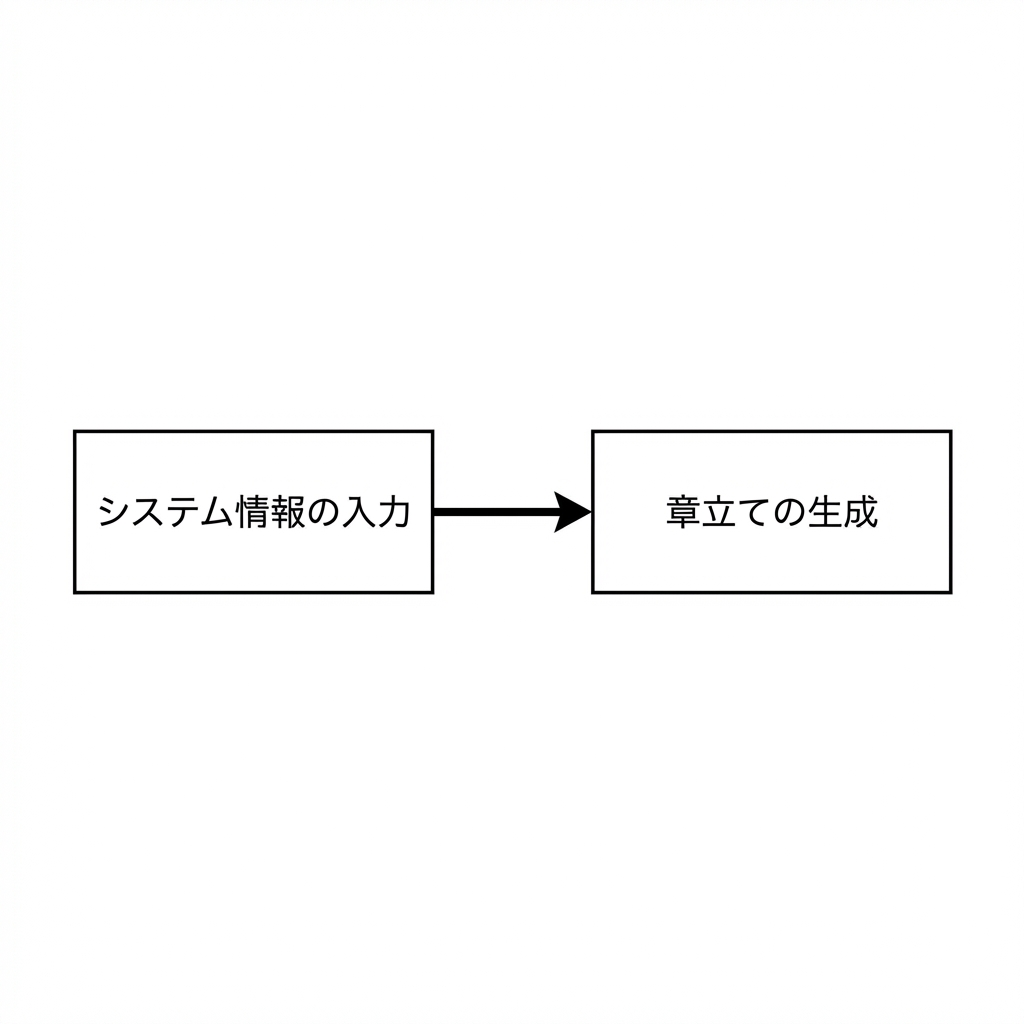
\includegraphics[width=0.8\linewidth]{./images/proposal_process_flow.png}
%   \caption{プロンプトの利用フロー}
%   \label{fig:process_flow}
% \end{figure}

\begin{enumerate}
    \item \textbf{システム情報の入力}:
    ユーザー（仕様書作成者）は、本プロンプトの「開発するシステム情報」欄に、対象システムの概要を記述する。また必要に応じて「システム仕様書の定義」の微調整を行う。

    \item \textbf{章立ての生成}:
    情報を入力したプロンプトをLLMに入力し、システム仕様書の章立てを生成させる。出力結果として、章・節・項の構造と、各章に記述すべき内容の指針が得られる。
\end{enumerate}

本研究では、このプロセスによって出力された章立てが、実用的なシステム仕様書の骨子として十分に機能するかを特に重視している。

次章以降では、本プロンプトを用いて実際に章立てを生成し、その網羅性や妥当性について評価を行う。


\iffalse
本章では、図、表、数式の挿入方法について説明する。

% \section{図の挿入}

図を挿入するには、\verb|figure| 環境と \verb|\includegraphics| コマンドを使用する。

% \subsection{基本的な図の挿入}

図\ref{fig:example}に例を示す。

\begin{figure}[tp]
  \centering
  \includegraphics[width=0.5\linewidth]{./images/syokuji_computer.png}
  \caption{図の挿入例}
  \label{fig:example}
\end{figure}

上記の図は以下のコードで挿入できる：

\begin{verbatim}
\begin{figure}[tp]
  \centering
  \includegraphics[width=0.5\linewidth]{./images/syokuji_computer.png}
  \caption{図の挿入例}
  \label{fig:example}
\end{figure}
\end{verbatim}

% \subsection{画像ファイルの配置}

画像ファイルは \verb|images/| ディレクトリに配置する。
サポートされている画像形式：PNG、JPG、PDF など。

% \section{表の挿入}

表を挿入するには、\verb|table| 環境と \verb|tabular| 環境を使用する。

% \subsection{基本的な表の挿入}

表\ref{tb:example}に例を示す。

\begin{table}[tp]
  \caption{表の挿入例}
  \label{tb:example}
  \centering
  \begin{tabular}{|l|c|r|}
    \hline
    左寄せ & 中央寄せ & 右寄せ \\
    \hline
    データ1 & データ2 & データ3 \\
    データ4 & データ5 & データ6 \\
    \hline
  \end{tabular}
\end{table}

上記の表は以下のコードで挿入できる：

\begin{verbatim}
\begin{table}[tp]
  \caption{表の挿入例}
  \label{tb:example}
  \centering
  \begin{tabular}{|l|c|r|}
    \hline
    左寄せ & 中央寄せ & 右寄せ \\
    \hline
    データ1 & データ2 & データ3 \\
    データ4 & データ5 & データ6 \\
    \hline
  \end{tabular}
\end{table}
\end{verbatim}

% \section{数式の挿入}

% \subsection{インライン数式}

文中に数式を挿入する場合は、\verb|$...$| または \verb|\(...\)| を使用する。
例：$E = mc^2$ は有名な公式である。

% \subsection{ディスプレイ数式}

独立した行に数式を表示する場合は、\verb|equation| 環境を使用する。

\begin{equation}\label{eq:example}
  \int_0^\infty e^{-x^2} dx = \frac{\sqrt{\pi}}{2}
\end{equation}

式(\ref{eq:example})のように、数式にも番号とラベルを付けて参照できる。

% \subsection{複数行の数式}

複数行の数式を表示する場合は、\verb|align| 環境を使用する：

\begin{align}
  a + b &= c \\
  x + y &= z
\end{align}

% \section{図表の参照}

図や表を参照するには、\verb|\ref{}| コマンドを使用する：

\begin{itemize}
  \item 図\ref{fig:example}のように図を参照
  \item 表\ref{tb:example}のように表を参照
  \item 式(\ref{eq:example})のように数式を参照
\end{itemize}
\fi